% Created 2026-04-23 四 23:40
% Intended LaTeX compiler: pdflatex
\documentclass[11pt]{article}
\usepackage[utf8]{inputenc}
\usepackage[T1]{fontenc}
\usepackage{graphicx}
\usepackage{longtable}
\usepackage{wrapfig}
\usepackage{rotating}
\usepackage[normalem]{ulem}
\usepackage{amsmath}
\usepackage{amssymb}
\usepackage{capt-of}
\usepackage{hyperref}
\date{\today}
\title{软件测试基础}
\hypersetup{
 pdfauthor={},
 pdftitle={软件测试基础},
 pdfkeywords={},
 pdfsubject={},
 pdfcreator={Emacs 30.2 (Org mode 9.7.11)}, 
 pdflang={English}}
\begin{document}

\maketitle
\tableofcontents

\section{总体观：软件测试围绕需求}
\label{sec:orgcf0d077}

测试围绕的中心是需求。测试不是单纯为了找bug，而是以用户需求为依据，判断产品是否符合需求；同时，测试也是 Verification 和 Validation 的统一：

\begin{itemize}
\item Verification: 产品有没有按照规格说明书正确实现
\item Validation: 产品是不是用户真正需要的东西
\end{itemize}


软件测试 = 基于需求，对软件进行检查和评价，发现它和预期之间的差距。

测试的直接任务是发现缺陷，根本目的是评价软件是否满足需求、保证质量。
\section{为什么要进行软件测试}
\label{sec:orge5c8a24}

\begin{enumerate}
\item 软件缺陷是客观存在的
\item 测试是质量保证中不可缺少的一环
\end{enumerate}


因为软件开发过程中会出现沟通误解、需求不完善、设计不合理、接口不匹配、边界考虑不周、算法与性能问题等，所以必须通过软件测试来尽早发现和控制这些缺陷。

\noindent\rule{\textwidth}{0.5pt}
\section{什么是软件缺陷，什么是软件质量保证}
\label{sec:org900c1da}
软件缺陷：软件产品中存在的问题，最终表现为用户需要的功能没有完全实现，不能满足或不能全部满足用户的需求。它的表现包括：功能没实现、性能不达标、结果不一致、运行出错、系统崩溃、界面混乱、用户不能接受等。

*软件缺陷的本质*：软件没有满足需求。

*软件缺陷的表现*：功能没实现、性能不达标、结果不符、行为异常、界面混乱等。

质量保证：为了确保软件开发过程和结果符合预期要求，而建立的一系列规程、活动和评价。也就是说，质量保证不只是最后只测一遍，而是靠全过程的规范、控制、改进和验证。

\begin{itemize}
\item 质量控制：盯过程，减少偏差
\item 质量保证：给出能够满足质量要求的证据
\item 软件测试：质量保证的重要手段，但不是全部
\end{itemize}


软件测试与质量保证的关系：软件测试时质量保证体系中的核心活动之一。质量保证覆盖开发过程与结果，测试则通过静态与动态的方法验证产品是否满足要求，并为质量保证提供依据。

\noindent\rule{\textwidth}{0.5pt}
\section{静态测试与动态测试}
\label{sec:org815dd31}
这很容易和黑盒测试、白盒测试混为一谈。
\subsection{静态测试}
\label{sec:orgd0538ca}
*不运行程序*。通过阅读、检查、分析来发现问题。需求评审、设计评审、代码评审放在静态测试里。
\subsection{动态测试}
\label{sec:org34333b2}
*运行程序*，观察输出、行为、状态，发现缺陷。黑盒测试和白盒测试都属于动态测试的主要方法。

\uline{静态测试看文档和代码，动态测试跑程序} 。

\noindent\rule{\textwidth}{0.5pt}
\section{黑盒测试与白盒测试}
\label{sec:org604270e}
\subsection{黑盒测试}
\label{sec:orge340ec7}
不看程序内部结构，只看输入和输出、功能和需求，依据需求规格说明书来设计测试。黑盒测试常用于功能验证、系统验证、验收测试。
\subsection{白盒测试}
\label{sec:org99cd041}
看程序内部结构，根据语句、分支、条件、路径等来设计测试，关注程序内部逻辑。白盒测试通常用于单元测试和集成测试。
\subsection{黑盒测试与白盒测试的关注点}
\label{sec:org3af611e}

\begin{itemize}
\item 黑盒：测功能有没有实现
\item 白盒：测内部逻辑有没有问题、覆盖够不够
\end{itemize}


\begin{itemize}
\item 等价类、边界值、因果图、决策表 →黑盒
\item 语句覆盖、判定覆盖、条件覆盖、基本路径 →白盒
\end{itemize}


\noindent\rule{\textwidth}{0.5pt}
\section{测试流程：从评审到验收}
\label{sec:orgec25b2b}
链路：\(需求评审 \rightarrow 设计评审 \rightarrow 单元测试 \rightarrow 集成测试 \rightarrow 功能验证测试 \rightarrow 系统测试 \rightarrow 验收测试\)，并伴随着测试计划、测试用例设计、测试执行、结果分析和报告。
\subsection{需求评审}
\label{sec:org4840f7e}
检查需求定义是否正确、完整、可测试、符合客户期望。
\subsection{设计评审}
\label{sec:org104c323}
检查系统设计是否合理、是否具有可测试性、是否满足性能、安全、扩展性等要求。
\subsection{单元测试}
\label{sec:org8ccf3fa}
测试最小单元，强调独立性，主要采用白盒，也可辅以黑盒；通常要用驱动模块和桩模块帮助测试。
\subsubsection{桩模块和驱动模块}
\label{sec:org094cbb0}
单元测试里，被测模块通常不能完全独立运行，所以通常需要调用“驱动模块”和“桩模块”来补齐测试环境。

驱动模块（driver）负责 *调用被测试模块*，用来模拟被测试模块的 *上级模块*。

驱动模块可以被理解为：发起调用的人，属于被测试模块的上游，主动把输入传入给被测模块，再返回接收结果、判断测试得对不对。

桩模块（stub），也叫存根程序，会模拟被 被测模块调用，用来模拟它依赖的下层模块。

桩模块是“假装成依赖的对象”。如果被测模块内部还需要去调用数据库、接口、别的函数，而那些函数还没有完成，或者不方便直接接入，就先用桩模块，返回一个预设好的结果。

\begin{itemize}
\item 驱动模块：模拟上游调用者
\item 桩模块：模拟下层被调用者
\end{itemize}
\subsection{集成测试}
\label{sec:org2115392}
把单元测试组装起来，重点发现接口问题和模块间协同问题。
\subsection{功能验证测试}
\label{sec:org9afff2e}
从用户角度验证系统是否正常实现，通常使用黑盒。
\subsection{系统测试}
\label{sec:org3f846bf}
把软件放到完整环境里测试，包括安装、容错、安全、压力、性能等。
\subsection{验收测试}
\label{sec:org7035c93}
发布前最后一次完整测试，核心特征是用户参与。

\noindent\rule{\textwidth}{0.5pt}
\section{V 模型}
\label{sec:org7eed056}

V模型是把“软件开发阶段”和“测试阶段”一一对应起来的模型。

\begin{figure}[htbp]
\centering
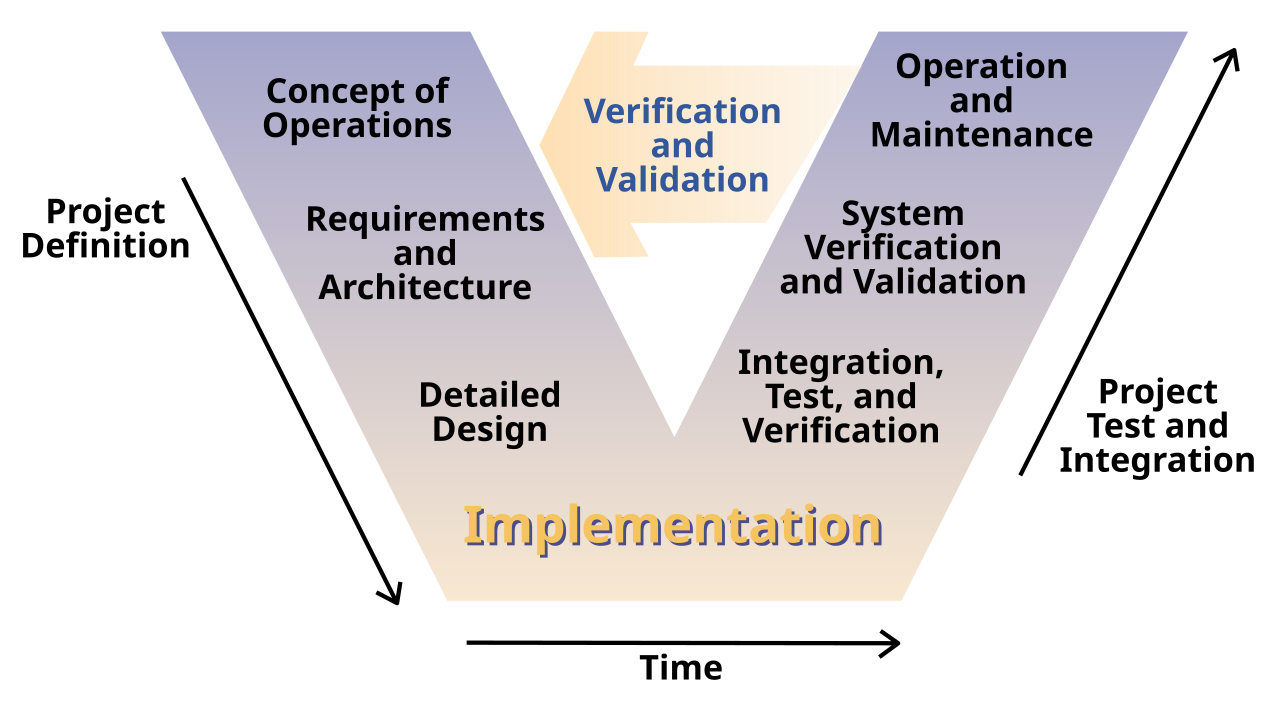
\includegraphics[width=.9\linewidth]{./v-model.png}
\caption{\label{fig:orga33f6b6}V 模型}
\end{figure}

左侧是：
\subsection{专案定义阶段}
\label{sec:org9442b5f}
\subsubsection{需求分析}
\label{sec:org688029c}
第一个阶段，也称为是验证（verification）阶段的第一个阶段。此阶段分析用户的需要，整理系统的需求（功能需求）。着重构建理想的系统，但不用决定软件的设计方式。
\subsubsection{系统设计}
\label{sec:orga5ae7c2}
系统设计师根据用户需求文件，分析并理解开发系统的业务流程的阶段。系统设计阶段会列出要实现用户需求需要的技术以及可能性。
\subsubsection{架构设计}
\label{sec:org9a5bb05}
该阶段会设计计算机系统架构及软件架构，选择架构的基准是应该可以实现所有模组的列表、模组的简单机能、界面关系等。
\subsubsection{模组设计}
\label{sec:orgc4dd794}
模组设计阶段也称为低阶设计。将设计的系统拆解为较小的单元或模组，并说明每一部分的内容，让程式设计者可以直接写程序。
\subsection{确认阶段}
\label{sec:orgbd80baf}
右侧是确认阶段。

V模型中，验证（或专案定义）阶段中的每一阶段，在确认阶段都会有对应的阶段。
\subsubsection{单元测试}
\label{sec:orgf9977a7}
模组设计 →单元测试。

单元测试的目的是要消除程序代码层级和单元层级的错误。单元是程序中可以独立存在的最小程序。
\subsubsection{集成测试}
\label{sec:org400f6a3}
架构设计 →集成测试。

集成测试的计划在架构设计阶段确定。集成测试会确认独立创建、独立测试过的模组是否可以共存和互相交互信息。
\subsubsection{系统测试}
\label{sec:orgabe4814}
系统设计 →系统测试。

系统测试计划会在系统设计的阶段确定。系统测试通常会由用户的团队来进行。系统测试会确保所开发的软件符合预期的需求，会测试整个程序的机能、相互依存以及通讯。系统测试也会验证系统符合的功能需求以及非功能需求。

负载测试、性能测试、压力测试、回归测试都是系统测试的一部分。
\subsubsection{验收测试}
\label{sec:orge099fc4}
需求分析→验收测试。

用户验收测试计划在需求分析阶段就确定。测试计划是由企业用户来进行。用户验收测试会在用户的环境下进行，设法模拟实际产品的环境，也会使用实际的数据。用户验收测试的目的是要确认所提供的系统符合客户需求，而且系统已经可以在实际环境下使用。

\noindent\rule{\textwidth}{0.5pt}
\section{需求评审和设计评审}
\label{sec:orgaae529a}

评审：对软件元素或项目状态进行评估，以判断是否与计划结果一致，并促进对其改进。评审可以是技术评审、文档评审、管理评审、流程评审。

需求评审的目标包括：
\begin{itemize}
\item 尽早发现需求问题，降低后期返工成本
\item 保证需求可测试
\item 让市场、产品、开发、测试对需求理解一直
\item 为测试计划和测试范围打基础
\end{itemize}


需求评审看什么：
\begin{itemize}
\item 正确性
\item 完备性
\item 一致性
\item 无二义性
\item 可验证性
\item 易追溯性
\end{itemize}


设计评审看什么：
\begin{itemize}
\item 稳定性、清晰性、合理性
\item 耦合度与内聚度
\item 数据与结构一致性
\item 可测试性、可追溯性
\item 安全性、性能、扩展性、可靠性
\end{itemize}


系统架构评审会关心单点故障、故障转移、负载均衡、关键业务设计是否合理；详细设计评审会看功能和接口定义、算法、数据流/控制流、模块独立性、可测试性。


\noindent\rule{\textwidth}{0.5pt}
\section{单元测试里必须记住的三个点}
\label{sec:org1a62835}
\subsection{单元测试的对象}
\label{sec:org761d30e}
针对软件最小单元，强调独立性，缩小问题范围。
\subsection{单元测试主要方法}
\label{sec:orgcf42cf2}
主要是白盒测试，辅以黑盒测试。白盒用于代码评审和逻辑覆盖，黑盒可用于较大单元的功能验证。
\subsection{驱动模块和桩模块}
\label{sec:org8f0de92}
\begin{itemize}
\item 驱动模块：模拟上级模块，负责调用被测模块
\item 桩模块：模拟下级模块，代替被测模块要调用的子模块
\end{itemize}


\noindent\rule{\textwidth}{0.5pt}
\section{速记}
\label{sec:org845dc04}

\begin{enumerate}
\item 测试围绕需求展开
\item 测试是Verificatio和Validation的统一
\item 静态测试不运行程序，动态测试运行程序
\item 黑盒测试看功能和输入输出，白盒测试看内部逻辑结构
\item 白盒测试常用于单元/集成，黑盒测试用于功能验证/系统/验收
\item 测试流程：\(需求评审 \rightarrow 设计评审 \rightarrow 单元测试 \rightarrow 集成测试 \rightarrow 功能验证 \rightarrow 系统测试 \rightarrow 验收测试\)
\item V 模型：单元测试和集成测试验证程序设计，系统测试验证系统设计，验收测试追溯用户需求
\item 单元测试常用驱动模块与桩模块辅助
\end{enumerate}
\end{document}
